\chapter{Introduction}
\label{chap:introduction}

\begin{center} % Abstract overview
\singlespacing\parbox{12cm}{\textit{
This chapter introduces the problem and motivation for the present master's thesis. It explains why pumped-storage hydropower with reversible pump-turbines (RPTs) is strategically important for a renewable-dominated electricity system. It identifies the cavitation barrier that limits pump-mode operation, and presents the booster-pump concept developed at NTNU under the name Store2Hydro. The hubless rim-driven thruster (RDT) is the candidate booster, and its strongly swirling outflow motivates a downstream guide-vane (GV) system. The thesis is then placed relative to the preceding project work~\cite{Leonsen2025}, and the scope is defined as a systematic CFD screening of guide-vane designs in the RDT--GV--draft-tube layout.
}}
\end{center}

\section{Background and motivation}
\label{sec:background_motivation}

The European electricity system is integrating a growing share of variable renewable generation. Balancing supply and demand on short timescales, rather than total installed capacity, is therefore becoming the binding constraint on system reliability~\cite{IEA_Renewables2023, EC_EGD_2021}. Among the available options, only hydropower with reservoirs and pumped-storage hydropower (PSH) provide flexibility at a scale relevant to a continental power system at acceptable cost~\cite{IRENA_Storage2017}.

Globally, 189~GW of pumped-storage capacity is installed, with a pipeline of new projects close to 600~GW~\cite{IHA_WHO_2025}. Norway holds a particular position in this landscape: hydropower accounts for roughly 90\,\% of national production~\cite{RegjeringenVannkrafthistorie2019}, and Norwegian reservoirs represent approximately half of the European hydropower storage capacity~\cite{NVE_Fleksibilitet2023}. This motivates the interest in upgrading existing Norwegian high-head plants for pumped-storage operation~\cite{DagsvikStorli2021}.

A cost-effective route is to retrofit the powerhouse with a reversible pump-turbine (RPT) instead of the original Francis runner~\cite{DagsvikStorli2021}. This reuses the existing waterways and reservoirs. The RPT operates as a Francis turbine in one direction and as a pump when rotation is reversed~\cite{Olimstad2012}. The dual-mode requirement is the central design tension of the machine. A runner well matched to turbine operation is rarely well matched to pump operation, and the cavitation limits in pump mode are stricter. Dagsvik's work shows that the available submergence in typical Norwegian high-head plants is often insufficient for an adequate net positive suction head (NPSH) margin in pump mode~\cite{DagsvikThesis2024}.

Cavitation is therefore a dominant hydraulic barrier to RPT retrofits at high-head sites~\cite{Franc2007}. IEC~60193 requires a clear NPSH margin between the available head and the head at which a 1\,\% efficiency drop occurs~\cite{IEC60193_2019}. Recent measurements on the NTNU RPT confirm that the cavitation margin is a limiting design parameter~\cite{Kerlefsen2025}. There are two alternatives that can overcome this constraint. The first is to lower the runner by excavating the powerhouse, but the civil works are typically prohibitive for an existing plant. The second is to install a booster pump in the draft tube upstream of the RPT, which raises the local pressure in pump mode without altering the civil structure~\cite{Valstad2018}. Earlier Store2Hydro work indicates that a booster of moderate head ($H \approx 5$~m) can provide the pressure increase required to improve the cavitation margin~\cite{Hage2020}.

The booster in this project has unusual constraints. It must fit inside a draft tube of diameter $\sim 0.5$~m. It must allow free passage when not in use. It must also not block reverse rotation in turbine mode. A conventional shaft-driven axial booster places obstacles in the centre of the duct. The hubless rim-driven thruster (RDT) places the electric motor in the duct rim and drives the blades through a rotating ring~\cite{Cao2012}. The hubless geometry leaves the centre of the duct open and is therefore well suited to draft-tube installation. Within Store2Hydro, the RDT has been adopted as the booster concept, and a sequence of project and master theses has developed its blade-element and 2D optimisation methodologies~\cite{Fjuk2025, Ambjornsson2025}.

%%%SETT INN BILDE AV RDT MOTOREN, BILDE FRA JOHANNES.

The RDT brings its own difficulty. As an axial-flow machine without a stator, the rotor leaves a strongly swirling and radially non-uniform wake at its discharge. Marine RDT studies show that the wake is dominated by helical tip and secondary vortices that persist many duct diameters downstream~\cite{Gaggero2023}. Without a downstream stator, a substantial part of the developed head is left in the flow as residual swirl~\cite{Andersen2014}. Axial pre-rotation at the RPT inlet affects both head and cavitation in pump mode. Positive pre-rotation reduces head and aggravates cavitation. Negative pre-rotation preserves head better but still reduces efficiency relative to swirl-free inflow~\cite{Jenssen2020, Larsen2019}. The natural design response is to place a row of stationary swirl-recovery guide vanes (GVs) downstream of the RDT. These are intended to reduce the residual swirl and recover part of the tangential kinetic energy as static pressure before the flow reaches the RPT runner.

\begin{figure}[h!]
  \centering
  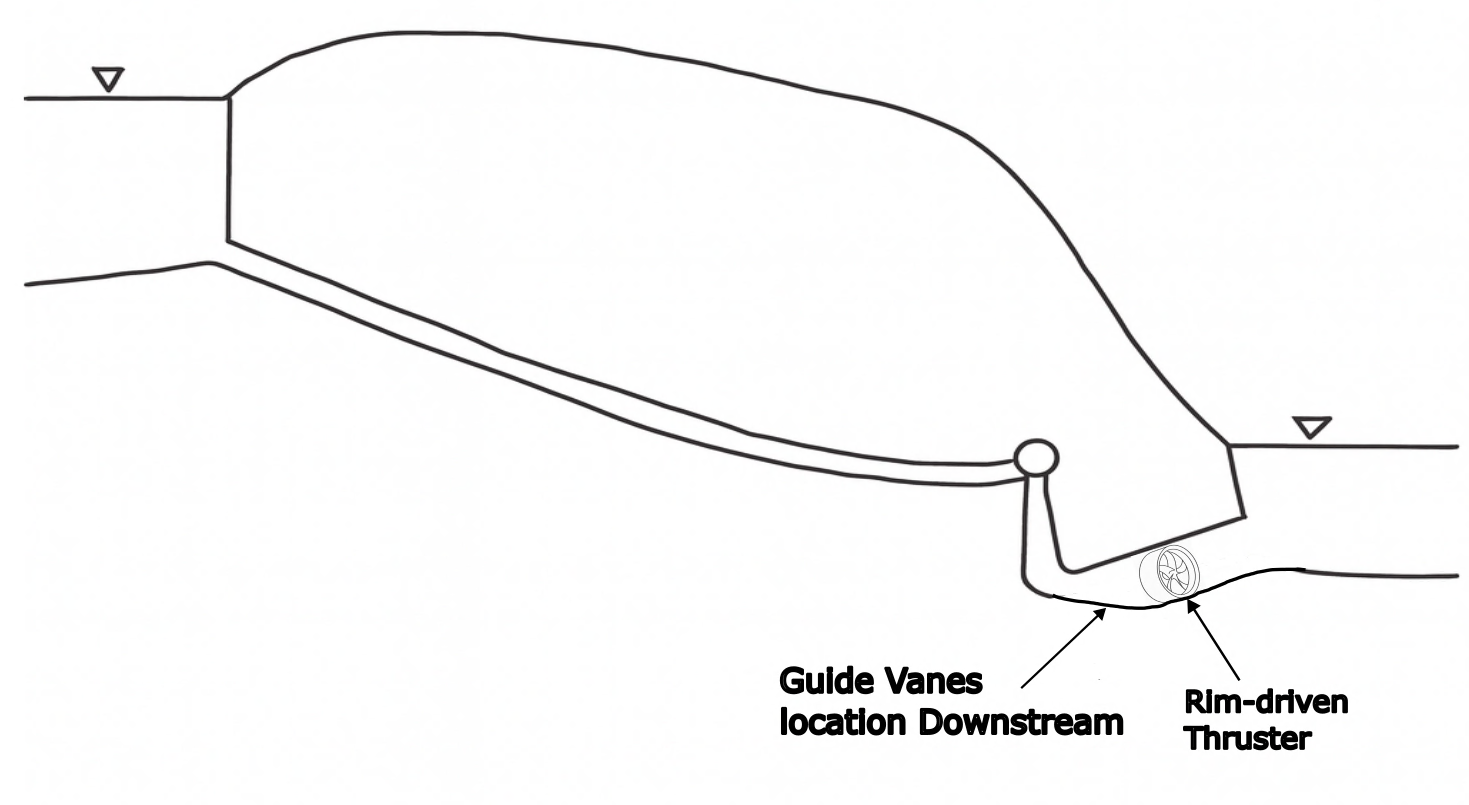
\includegraphics[width=0.75\textwidth]{Figures/Litterature_review/Sketch_RDT_GV.png}
  \caption[Concept sketch of the RDT--GV booster system]{Concept sketch of the RDT booster with a downstream GV row in the draft tube of a reversible pump-turbine retrofit. Adapted from the project work~\cite{Leonsen2025}.}
  \label{fig:concept_intro}
\end{figure}

\section{Project work and the gap addressed by this thesis}
\label{sec:project_work_gap}

The present thesis is a direct continuation of the project work \emph{Parametric Hydraulic Design of Guide Vanes for a Rim-Driven Thruster in Pumped-Storage Hydropower}~\cite{Leonsen2025}. The project work delivered three contributions. The first is a parametric MATLAB tool, \texttt{vanedesign\_loft\_export}, that generates NACA-type GV sections and exports 3D geometries for CAD and CFD. The second is a CFD-based slip database condensed into a response-surface model. The third is a first comparative CFD study of two GV geometries (Case~A and Case~B) in a short straight duct, demonstrating the trade-off between swirl reduction and total-pressure loss.

This starting point falls short in three respects. First, only two 3D geometries were assessed with CFD. Two data points indicate a trade-off, but they do not map the design space. The project work explicitly lists this limited screening as a gap to close in further work~\cite{Leonsen2025}. Second, the project-work CFD domain was a straight pipe. It did not include the conical contraction, the $90^\circ$ bend, and the final inlet section present in the actual Store2Hydro layout. Third, the parallel RPT pump-mode simulations by Dokset~\cite{Dokset2025} used inlet profiles extracted \emph{downstream} of the GVs. The reported RPT performance numbers therefore do not include the GV passage drag. The configuration that gives the most favourable RPT inflow is therefore not automatically the one that gives the best full-system behaviour.

The present thesis addresses the first two gaps directly. The slip-correction methodology from~\cite{Leonsen2025} is reused with a single fixed value $\delta_{\mathrm{TE}} = 6^\circ$. This follows G\"ulich's recommendation~\cite{Gulich2010} that a small built-in TE angle of $4^\circ$--$6^\circ$ is sufficient to compensate for cascade deviation while avoiding the separation risk of aggressive correction. The screening then simulates 18 GV configurations in the full RDT--GV--draft-tube domain. The matrix combines two chord-control strategies (constant chord and constant solidity at the shroud), six shroud-chord levels and three vane counts. A nineteenth simulation, denoted \texttt{NoGV}, replaces the GV region with an empty pipe and provides the reference for the swirl-reduction and head-loss metrics. The third gap (coupling with the RPT) is left as future work. Dokset~\cite{Dokset2025} carries the parallel responsibility for the RPT side, and a coupled RDT--GV--RPT campaign exceeds the available computational budget.

\section{Goal and research questions}
\label{sec:goal_research_q}

The main goal of this thesis is

\medskip
\begin{quote}
\textit{To develop a systematic CFD screening methodology for swirl-recovery guide vanes downstream of the rim-driven thruster in the Store2Hydro booster--RPT concept. The methodology is then used to identify how the dominant design variables govern the trade-off between swirl reduction, hydraulic loss, and downstream flow quality through the conical section, the $90^\circ$ bend, and the final inlet section before the RPT.}
\end{quote}
\medskip

This goal is broken down into four research questions:
\begin{enumerate}
  \item How do GV design parameters --- vane count $Z_s$, chord-control strategy (CC vs CS), and shroud-chord magnitude --- influence swirl reduction, residual swirl distribution and total-pressure loss in the integrated RDT--GV--draft-tube system?
  \item Which spanwise and plane-averaged metrics best discriminate between GV designs that condition the inflow well for the RPT and designs that do not?
  \item Is the design with the lowest residual tangential velocity directly downstream of the GVs also the design with the most favourable inflow at the bend exit? Or does the bend redistribute residual swirl in a way that changes the ranking?
  \item How robust is the design ranking when evaluated across several axial planes between the GVs and the RPT inlet, and what mechanism limits the achievable swirl reduction in this geometry?
\end{enumerate}

A working hypothesis is formulated for each question. It is hypothesised that increasing solidity (longer chord or higher vane count) reduces residual swirl monotonically but at a cost in total-pressure loss. The best designs will therefore lie on a Pareto front rather than at the extreme of maximum swirl recovery. Residual swirl is further hypothesised to interact measurably with the bend secondary flow. Designs with similar swirl numbers immediately downstream of the GVs may therefore differ markedly in inflow quality at the bend exit.

\section{Scope and limitations}
\label{sec:scope_limitations}

The scope is constrained by previous work and by the available computational resources. Three explicit decisions define the boundary.

\paragraph{Decoupling from the RPT.} The simulation domain extends from the RDT inlet through the RDT, the GV row, the conical contraction from $D = 0.5$~m to $D = 0.4$~m, the $90^\circ$ bend, and a straight final pipe of length $\sim 1.0$~m towards the RPT. The RPT itself is replaced by this final pipe. The pipe acts as a buffer to reduce the influence of the imposed outlet boundary condition on the post-bend flow field. A coupled RDT--GV--RPT screening over 18 configurations was estimated to exceed the available time-frame by a factor of approximately three. The decision is justified in detail in Section~\ref{sec:rpt-decoupling-justification}.

\paragraph{Single operating point.} All 18 configurations and the \texttt{NoGV} reference are simulated at $\dot m = 290.3$~kg/s and $n = 650$~rpm. Off-design behaviour is not investigated. The goal is comparative ranking of GV geometries at one representative operating point.

\paragraph{Steady RANS for the screening.} The 18-case screening uses steady RANS with the SST $k$--$\omega$ turbulence model. Two transient simulations of selected configurations are included for the rotor--stator interaction analysis (Chapter~\ref{chap:results_discussion}). A full transient screening campaign is not feasible in the time-frame.

\medskip
The following limitations from the project work are inherited:
\begin{itemize}
  \item the RDT wake used to design the GVs corresponds to a single RDT geometry and operating point, taken from the data sets \texttt{shubham\_blade6} and \texttt{shubham\_transient};
  \item cavitation is not modelled in the screening campaign and is treated only indirectly through the static-pressure field;
  \item structural strength, fatigue and vibration of the GVs are not analysed beyond the unsteady-loading diagnostics in Chapter~\ref{chap:results_discussion};
  \item the slip correction is fixed at $\delta_{\mathrm{TE}} = 6^\circ$ rather than swept across designs.
\end{itemize}

The thesis should therefore be read as a structured screening study. It reduces a large design space to a small number of credible candidates. It also quantifies the dominant trade-off between swirl reduction and total-pressure loss. A coupled RDT--GV--RPT simulation, cavitation assessment and final experimental validation of the shortlisted design are listed as future work in Chapter~\ref{chap:future_work}.

\section{Thesis outline}
\label{sec:thesis_outline}

The thesis is organised as follows. Chapter~\ref{chap:litterature} reviews the literature on rim-driven thrusters, swirling pipe flow, GV design, slip correlations, swirl decay, and secondary flow in curved ducts. Chapter~\ref{chap:theory_method} consolidates the theoretical framework and the design methodology. It covers the governing equations, swirl metrics, cascade theory, Dean-vortex theory of the $90^\circ$ bend, and rotor--stator interaction theory. The same chapter presents the 18-case design matrix, the parametric MATLAB workflow, the multi-domain CFX setup, the mesh and Grid Convergence Index study, the analysis-plane definitions, and the spectral-analysis methodology. Chapter~\ref{chap:results_discussion} presents the simulation results, including the spanwise diagnostics and the unsteady rotor--stator analysis of the two transient runs. Chapter~\ref{chap:conclusion} concludes and Chapter~\ref{chap:future_work} states the recommended directions for future work.

\clearpage